% Рисунок из тетради: область Ω внутри куба Q = (0,d)^n.
\begin{figure}[htbp]
\centering
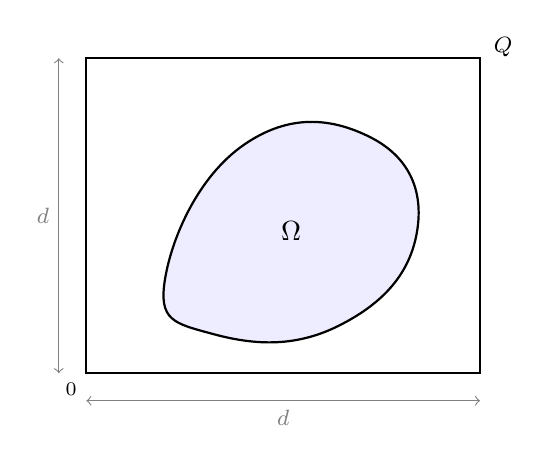
\begin{tikzpicture}[scale=1.0]
  \draw[thick] (0,0) rectangle (5,4);
  \node[anchor=south west, font=\footnotesize] at (5.05,3.9) {$Q$};

  \draw[thick, fill=blue!7]
    plot[smooth cycle, tension=0.8]
      coordinates {(1.0,1.2) (2.0,2.9) (3.6,3.0) (4.2,1.8) (3.2,0.6) (1.6,0.5)};
  \node at (2.6,1.8) {$\Omega$};

  \draw[<->, gray] (0,-0.35) -- node[below, font=\footnotesize]{$d$} (5,-0.35);
  \draw[<->, gray] (-0.35,0) -- node[left, font=\footnotesize]{$d$} (-0.35,4);

  \node[anchor=north east, font=\scriptsize] at (0,0) {$0$};
\end{tikzpicture}
\caption{К неравенству Фридрихса: область $\Omega$ помещается в куб
$Q = (0,d)^n$ со стороной $d = \operatorname{diam}\Omega$. Функция
$u \in C_0^\infty(\Omega)$, продолженная нулём, обращается в нуль на всей грани
$x_n = 0$, что и позволяет написать $u(x) = \int_0^{x_n} \partial_n u\, dt$.}
\label{fig:cube-omega}
\end{figure}
